\section{Introduction}
\label{sec:intro}


Symbolic model checking using induction-based techniques such as IC3/PDR~\cite{Een2011:PDR} and $k$-induction~\cite{SheeranSS00} can often determine whether safety properties hold of complex finite or infinite-state systems.  Model checking tools are attractive both because they are automated, requiring little or no interaction with the user, and if the answer to a correctness query is negative, they provide a counterexample to the satisfaction of the property.  These counterexamples can be used both to illustrate subtle errors in complex hardware and software designs~\cite{hilt2013,McMillan99:compositional, Miller10:CACM} and to support automated test case generation~\cite{Whalen13:OMCDC, You15:dse}.
In the event that a property is proved, however, it is not always clear what level of assurance should be invested in the result.  Given that these kinds of analyses are performed for safety- and security-critical software, this can lead to overconfidence in the behavior of the fielded system.  It is well known that issues such as vacuity~\cite{Kupferman03:Vacuity} can cause verification to succeed despite errors in a property specification or in the model. Even for non-vacuous specifications, it is possible to over-constrain the specification of the {\em environment} in the model such that the implementation will not work in the actual operating environment.

At issue is the level of feedback provided by the tool to the user. In
most tools, when the answer to a correctness query is positive, no
further information is provided. What we would like to provide is
traceability information, an {\em inductive validity core} (IVC), that explains
the proof, in much the same way that a counterexample explains the
negative result. This is not a new idea: UNSAT cores~\cite{zhang2003extracting}
provide the same kind of information for individual SAT or
SMT queries, and this approach has been lifted to bounded analysis
for Alloy in~\cite{Torlak08:cores}. What we propose is a generic and efficient
mechanism for extracting supporting information, similar to an UNSAT
core, from the proofs of safety properties using inductive techniques
such as PDR and $k$-induction. Because many
properties are not themselves inductive, these proof techniques
introduce lemmas as part of the solving process in order to strengthen
the properties and make them inductive. Our technique allows
efficient, accurate, and precise extraction of inductive validity cores
even in the presence of such auxiliary lemmas.

Once generated, the IVC can be used for many purposes in the software verification process, including at least the following:
\begin{description}
    \item[Vacuity detection:] The idea of syntactic vacuity detection (checking whether all subformulae within a property are necessary for its satisfaction) has been well studied~\cite{Kupferman03:Vacuity}.   However, even if a property is not syntactically vacuous, it may not require substantial portions of the model.  This in turn may indicate that either a.) the model is incorrectly constructed or b.) the property is weaker than expected.  We have seen several examples of this mis-specification in our verification work, especially when variables computed by the model are used as part of antecedents to implications.
    \item[Completeness checking:] Closely related to vacuity detection is the idea of {\em completeness checking}, e.g., are all atoms in the model necessary for at least one of the properties proven about the model?  Several different notions of completeness checking have been proposed~\cite{chockler_coverage_2003, kupferman_theory_2008}, but these are very expensive to compute, and in some cases, provide an overly strict answer (e.g., checking can only be performed on non-vacuous models for~\cite{kupferman_theory_2008}). %\ela{Mike, as you said there must be different definitions for completeness. But, the one you mentioned here as an example, I think, is not exactly what we want. I would say,} \fixed{e.g., are all atoms in the model necessary for the properties proven about the model?}  \ela{  Also, the next sentence gives somehow the impression that those definitions are very good, but expensive. Instead, ours is only cheap. It does not say ours is better. I would change it like this:  } \fixed{In~\cite{chockler_coverage_2003, kupferman_theory_2008}, several different notions of completeness checking have been proposed that are rather practical to compute, and in some cases, provide an overly strict answer (e.g., checking can only be performed on non-vacuous models for~\cite{kupferman_theory_2008}). However, as an added benefit, the IVC idea not only lowers the computational cost, but also introduces a novel way of checking completeness for free.}    \ela{BUT, maybe not SO good to claim this in this paper becuz we don't have enough supporting evidence}
% TODO: \mike{Double check this! (for kupferman_theory_2008)}
    \item[Traceability:] Certification standards for safety-critical systems (e.g.,~\cite{DO178C, MOD:00-55}) usually require {\em traceability matrices} that map high-level requirements to lower-level requirements and (eventually) leaf-level requirements to code or models.  Current traceability approaches involve either manual mappings between requirements and code/models~\cite{SimulinkTraceability} or a heuristic approach involving natural language processing~\cite{Keenan12:Tracelab}.  Both of these approaches tend to be inaccurate.  For functional properties that can be proven with inductive model checkers, inductive validity cores can provide accurate traceability matrices with no user effort.
    \item[Symbolic Simulation / Test Case Generation:]  Model checkers are now often used for symbolic simulation and structural-coverage-based test case generation~\cite{SimulinkDesignVerifier,Whalen13:OMCDC}.  For either of these purposes, the model checker is supposed to produce a witness trace for a given coverage obligation using a ``trap property'' which is expected to be falsifiable.  In systems of sufficient size, there is often ``dead code'' that cannot ever be reached.  In this case, a proof of non-reachability is produced, and the IVC provides the reason why this code is unreachable.
\end{description}
\noindent Nevertheless, to be useful for these tasks, the generation
process must be efficient and the generated IVC must be
accurate and precise (that is, sound and close to minimal).  The requirement for accuracy is obvious; otherwise the ``minimal'' set of model elements is no longer sufficient to produce a proof, so it no longer meets our IVC definition.  Minimality is important because (for traceability) we do not want unnecessary model elements in the trace matrix, and (for completeness) it may give us a false level of confidence that we have enough requirements.

%\ela{should we add this: (?)}
In addition, %\fixed{ a property can have as many unique minimal IVC sets as the possible paths through which it can be proved. Therefore,}
we are also interested in {\em diversity}:  how many different IVCs can be computed for a given property and model? Requirements engineers often talk about ``the traceability matrix'' or ``the satisfaction argument''.  If proofs are regularly diverse, then there are potentially many equally valid traceability matrices, and this may lead to changes in traceability research.

%% We put the image here so it shows up side-by-side with fig:ex-after
\begin{figure}[t]
\centering
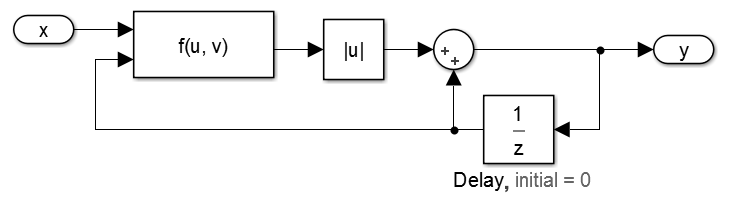
\includegraphics[width=\columnwidth]{figs/simulink.png}
{\smaller
\begin{verbatim}
node filter(x : real) returns (a, b, y : real);
let
  a = f(x, 0.0 -> pre y);
  b = if a >= 0.0 then a else -a;
  y = b + (0.0 -> pre y);
tel;
\end{verbatim}
}
\vspace{-0.1in}
\caption{Model with property $y \geq 0$, before IVC analysis}
\label{fig:ex-before}
\end{figure}

In the remainder of this paper, we present an algorithm for efficient generation of IVCs for induction-based model checkers.  Our contributions, as detailed in the remainder of the paper, are as follows:

\begin{itemize}
    \item We present a technique for extracting inductive validity
      cores from an inductive verification of a safety property over a sequential model involving lemmas.
    \item We formalize this technique and present an implementation of it in the JKind model checker~\cite{jkind}.
    \item We present an experiment over our implementation and measure the efficiency, minimality, and robustness of the IVC generation process.
\end{itemize}

The rest of this article is organized as follows. In
Section~\ref{sec:exmpl}, we present a motivating example. In
Section~\ref{sec:background}, we present the required background for
our approach. In Sections~\ref{sec:ivc} and~\ref{sec:impl}, we present
our approach and our implementation in JKind.
Sections~\ref{sec:experiment} and~\ref{sec:results} present an
evaluation of our approach on a set of benchmark examples. Finally,
Section~\ref{sec:related} discusses related work and
Section~\ref{sec:conc} concludes.

\iffalse
\begin{itemize}
    \item Overview of the problem: sequential model checkers do not provide much insight into proofs.
    \item Section should roughly follow the structure of "Finding Minimal Unsatisfiable Cores of
        Declarative Specifications" paper by Torlak et al (with Dan Jackson).
    \item UNSAT Cores have been used for a variety of analysis tasks
    \item we want to generalize this idea for sequential systems
\end{itemize}
\fi

%%% Local Variables:
%%% mode: latex
%%% TeX-master: "main.tex"
%%% End

%%  LocalWords:  IC PDR IVC UNSAT subformulae mis IVCs Torlak et al
